\documentclass[a4paper,UTF8]{ctexart}
\usepackage{graphicx}
\usepackage{geometry}
\usepackage{xcolor}
\usepackage{amsmath}
\usepackage{enumerate}
\usepackage{caption}
\usepackage{listings}
\usepackage{array}
\usepackage{booktabs}
\usepackage{tikz}
\usetikzlibrary{shapes,arrows}
\usepackage{pgfplots}
\pgfplotsset{compat=1.17}
\usepackage{appendix}
\captionsetup[lstlisting]{labelfont=bf,justification=justified}
\usepackage{multicol}
\setlength{\columnsep}{3em}
\usepackage{float}

\graphicspath{{img/}}

\usepackage[colorlinks,linkcolor=blue]{hyperref}
\usepackage{bookmark}
\providecommand{\code}[2]{\lstinputlisting[language=#2,caption=\href{run:#1}{\ttfamily #1}]{#1}}
\providecommand{\img}[1]{\includegraphics[width=0.88\textwidth]{#1}}

% listings
\definecolor{grey}{rgb}{0.8,0.8,0.8}
\definecolor{darkgreen}{rgb}{0,0.3,0}
\definecolor{darkblue}{rgb}{0,0,0.3}
\lstset{%
    numbers=left, %行号
    numberstyle=\scriptsize\color{grey},
    showstringspaces=false,
    showspaces=false,%
    tabsize=4,%
    frame=shadowbox,%
    basicstyle={\ttfamily\normalsize},%
    keywordstyle=\color{blue!80!black}\bfseries,%
    identifierstyle=,%
    commentstyle=\color{green!50!blue}\itshape,%
    stringstyle=\color{green!50!black},%
    rulesepcolor=\color{gray!20!white},
    breaklines,
    columns=flexible,
    extendedchars=false,
    %mathescape=true,
    language=verilog,
}

\begin{document}
\title{\normalsize \underline{计算机系统结构实验}\\\LARGE 实验 4 报告\\\vspace*{1em}\normalsize 简单的类 MIPS 单周期处理器\\部件实现--寄存器、存储器与有符号扩展}
\author{李子龙\\ 518070910095}
\date{\today}
\maketitle
\tableofcontents
\clearpage

\section{实验目的}

\begin{enumerate}
    \item 理解CPU的寄存器、存储器、有符号扩展
    \item Register的实现
    \item DataMemory的实现
    \item 有符号扩展的实现
    \item 使用行为仿真
\end{enumerate}

\section{原理分析}

\subsection{寄存器堆}

寄存器堆是指令操作的主要对象。5 位的 \verb"readReg1",\verb"readReg2",\verb"writeReg" 将用于指定需要的寄存器地址,即访问 32($=2^5$) 个寄存器的其中一个。在时钟下沿,并且 \verb"regWrite" 变为可用时,才会写入数据。(在这里规定均在时钟下沿写入数据,这样才不会读取错误的数据)读取得到的数据将会通过 \verb"readData1" 和 \verb"readData2" 输出。

\begin{figure}[h]
    \centering
    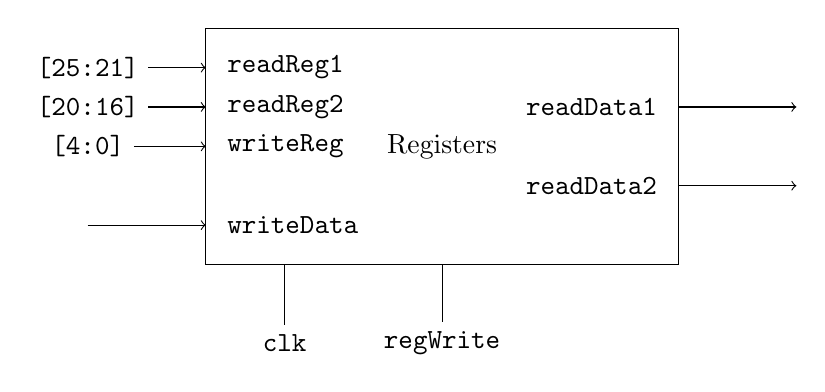
\begin{tikzpicture}
\tikzstyle{io}=[font=\ttfamily];
\tikzstyle{lio}=[io,right,xshift=-1em];
\tikzstyle{rio}=[io,left,xshift=1em];

\draw  (-1.5,2) rectangle (4.5,-1);
\node[lio] at (-1,1.5) {readReg1};
\node[lio] at (-1,1) {readReg2};
\node[lio] at (-1,0.5) {writeReg};
\node[lio] at (-1,-0.5) {writeData};
\node[io] (v2) at (1.5,-2) {regWrite};
\node[rio] at (4,1) {readData1};
\node[rio] at (4,0) {readData2};
\node[io] (v1) at (-0.5,-2) {clk};
\draw (v1) -- (-0.5,-1);
\draw (v2) -- (1.5,-1);

\draw (-3,1.5) node [io] {[25:21]} edge[->] (-1.5,1.5);
\draw (-3,1) node [io] {[20:16]} edge[->] (-1.5,1);
\draw (-3,0.5) node [io] {[4:0]} edge[->] (-1.5,0.5);
\draw (-3,-0.5) edge[->] (-1.5,-0.5);
\draw (4.5,1) edge[->] (6,1);
\draw (4.5,0) edge[->] (6,0);
\node at (1.5,0.5) {Registers};
\end{tikzpicture}
    \caption{寄存器堆模块}
\end{figure}

\subsection{内存单元模块}

内存模块获取 32 位地址 \verb"address" 的输入。读写控制信号是独立的,一个时钟周期最多激活存储器读 \verb"memRead" 和存储器写 \verb"memWrite" 中的其中一个。需要写入的数据通过 \verb"writeData" 获取,输出的数据从 \verb"readData" 输出。

\begin{figure}[h]
    \centering
    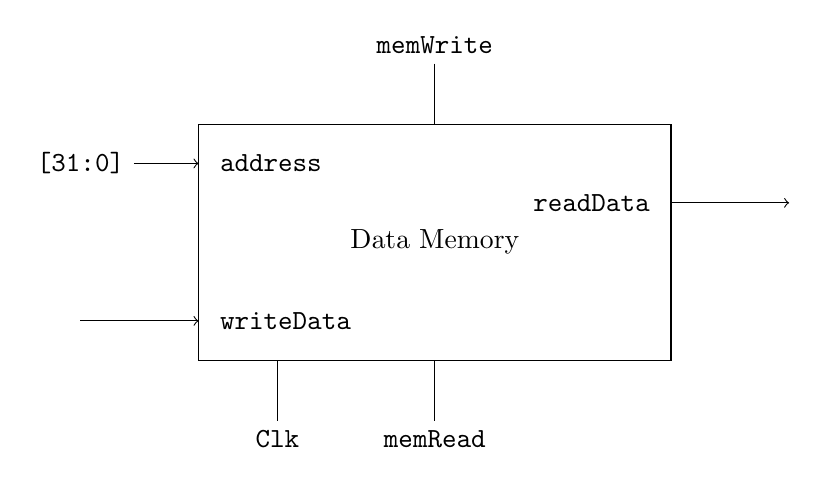
\begin{tikzpicture}
\tikzstyle{io}=[font=\ttfamily];
\tikzstyle{lio}=[io,right,xshift=-1em];
\tikzstyle{rio}=[io,left,xshift=1em];

\draw  (-1.5,2) rectangle (4.5,-1);
\node[lio] at (-1,1.5) {address};
\node[lio] at (-1,-0.5) {writeData};
\node[io] (v2) at (1.5,-2) {memRead};
\node[rio] at (4,1) {readData};
\node[io] (v1) at (-0.5,-2) {Clk};
\draw (v1) -- (-0.5,-1);
\draw (v2) -- (1.5,-1);

\draw (-3,1.5) node [io] {[31:0]} edge[->] (-1.5,1.5);
\draw (-3,-0.5) edge[->] (-1.5,-0.5);
\draw (4.5,1) edge[->] (6,1);
\node at (1.5,0.5) {Data Memory};
\node[io] (v3) at (1.5,3) {memWrite};
\draw (v3) -- (1.5,2);
\end{tikzpicture}
    \caption{内存模块}
\end{figure}

\subsection{带符号扩展}

将 16 位数符号扩展为 32 位的符号数。

\begin{figure}[H]
    \centering
    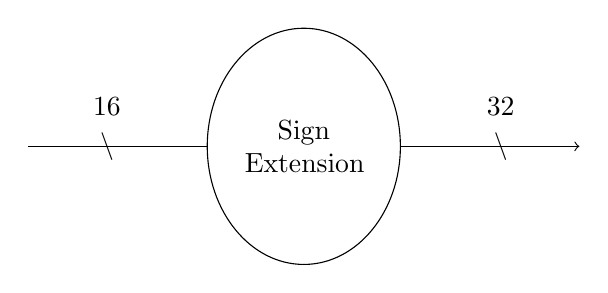
\begin{tikzpicture}[node distance=0.5cm]
\draw (-3.5,0) edge[->] (3.5,0);
\node [ellipse,draw,text width=1.5cm,text centered,minimum height=3cm,fill=white] at (0,0) {Sign\\Extension};
\node (v1) at (-2.5,0) {$\backslash$};
\node [above of=v1] {16};
\node (v2) at (2.5,0) {$\backslash$};
\node [above of=v2] {32};
\end{tikzpicture}
    \caption{带符号扩展}
\end{figure}

\section{代码实现}

\subsection{寄存器堆}

32 位的 MIPS 中共有 32 个 32 位的寄存器,在寄存器内部用下面的语句表示。
\begin{lstlisting}
    reg [31:0] RegFile [31:0];
\end{lstlisting}

按照原理,安排读取语句和写入语句。
\begin{lstlisting}[caption=Registers.v]
    reg [31:0] RegFile [31:0];
    reg [31:0] ReadData1;
    reg [31:0] ReadData2;

    always @(readReg1 or readReg2) begin
        ReadData1 = RegFile[readReg1];
        ReadData2 = RegFile[readReg2];
    end
    
    always @(negedge clk) begin
        if(regWrite)
            RegFile[writeReg] = writeData;
    end

    assign readData1 = ReadData1;
    assign readData2 = ReadData2;
\end{lstlisting}

\subsection{内存单元模块}

如果是读数据,如果 \verb"memRead" 被激活或者地址发生了改变,首先会判断地址是否在物理地址空间内(这里存储器只有 64 个,地址空间却为 32 位),如果是就会从 \verb"readData" 输出数据;否则是无效地址将清空读到的数据;如果是写数据,如果 \verb"memWrite" 被激活,而且在物理地址空间内,则会在时钟下沿从 \verb"writeData" 读取数据,并写入寄存器。

\begin{lstlisting}[caption=dataMemory.v]
    reg [31:0] MemFile[0:63];

    always @(memRead or address) begin
        if(address<31'h00000020)
            readData = MemFile[address];
        else 
            readData = 31'h00000000;
    end

    always @(negedge Clk) begin
        if(memWrite && address<31'h00000020)
            MemFile[address] = writeData;
    end
\end{lstlisting}

\subsection{带符号扩展}

这里采用了扩展复制第一位至前16位的方法进行符号扩展。

\begin{lstlisting}[caption=signext.v]
    assign data = {{16 {inst[15]}},inst[15:0]};
\end{lstlisting}

\section{仿真结果}

\subsection{寄存器堆}

寄存器堆的激励文件如下。时钟周期被设定为 100ns。
    \begin{lstlisting}[caption=Registers\_tb.v,basicstyle=\ttfamily\scriptsize]
        initial begin
            readReg1 = 0;
            readReg2 = 0;
            writeReg = 0;
            writeData = 0;
            regWrite = 0;
            clk = 0;
    
            #285;
            regWrite = 1'b1;
            writeReg = 21;
            writeData = 32'b11111111111111110000000000000000;
    
            #200;
            writeReg = 10;
            writeData = 32'b00000000000000001111111111111111;
    
            #200;
            regWrite = 1'b0;
            writeReg = 0;
            writeData = 32'b00000000000000000000000000000000;
    
            #50;
            readReg1 = 5'b10101;
            readReg2 = 5'b01010;
        end
    \end{lstlisting}

图 \ref{fig:regs} 显示了仿真结果。在时钟下沿稳定写入信号,向地址 21 写入 \verb"FFFF0000" ,向地址 10 写入 \verb"0000FFFF",然后读取地址 21 和 10 的数据,分别为 \verb"FFFF0000" 和 \verb"0000FFFF" 输出到 \verb"readData1" 和 \verb"readData2"。

% TODO: 或许重写激励的时钟
\begin{figure}[h]
    \centering
    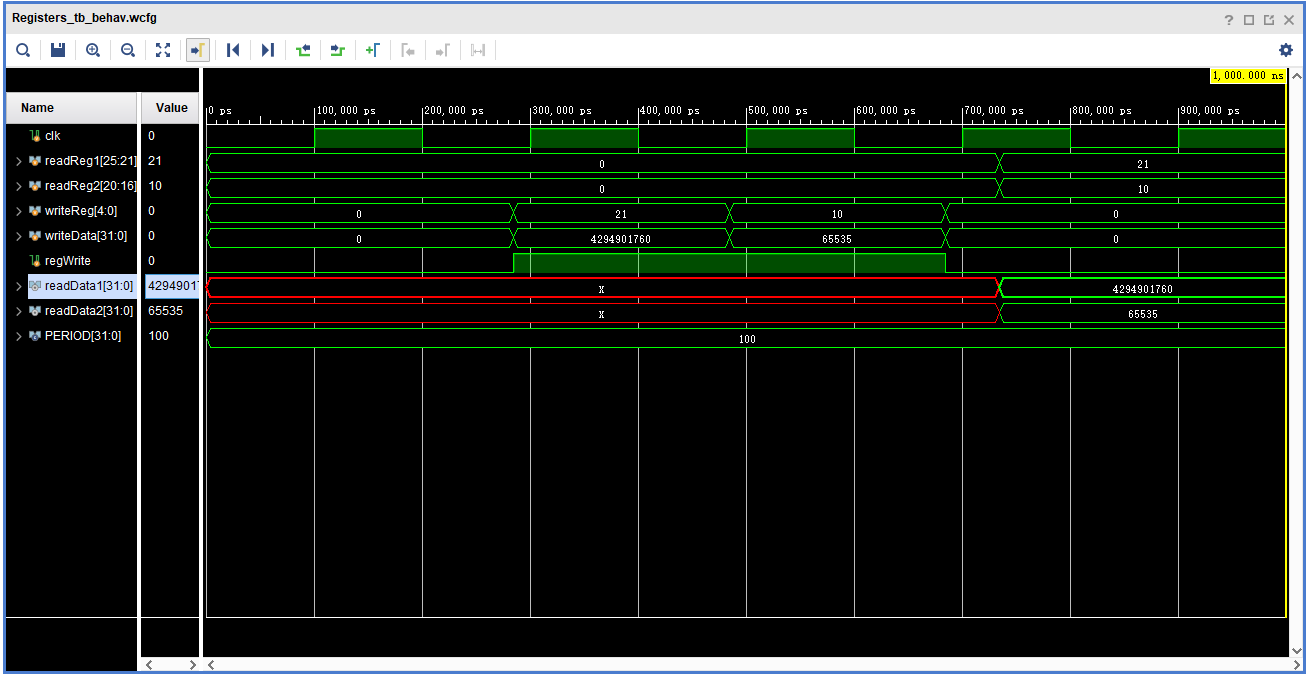
\includegraphics[width=\textwidth]{figure1.png}
    \caption{寄存器堆的仿真结果}
    \label{fig:regs}
\end{figure}

\subsection{内存单元模块}

内存单元模块的激励文件如下。
    \begin{lstlisting}[caption=dataMemory\_tb.v,basicstyle=\ttfamily\scriptsize]
        initial begin
            address = 0;
            writeData = 0;
            Clk = 0;
            memWrite = 0;
            memRead = 0;
    
            #185;
            memWrite = 1'b1;
            address = 32'b00000000000000000000000000000111;
            writeData = 32'b11100000000000000000000000000000;
    
            #100;
            memWrite = 1'b1;
            writeData = 32'hffffffff;
            address = 32'b00000000000000000000000000000110;
    
            #185;
            memRead = 1'b1;
            memWrite = 1'b0;
            address = 32'b00000000000000000000000000000111;
    
            #80;
            memWrite = 1;
            address = 8;
            writeData = 32'haaaaaaaa;
    
            #80;
            memWrite = 0;
            memRead = 1;
            address = 6;
        end
    \end{lstlisting} 

内存模块的仿真结果如图 \ref{fig:memtb} 所示。在后面的读取数据时,地址 7 读到了之前写入的 \verb"e0000000",地址 6 读到了之前写入的 \verb"aaaaaaaa"。仿真结果是正确的。
\begin{figure}[h]
    \centering
    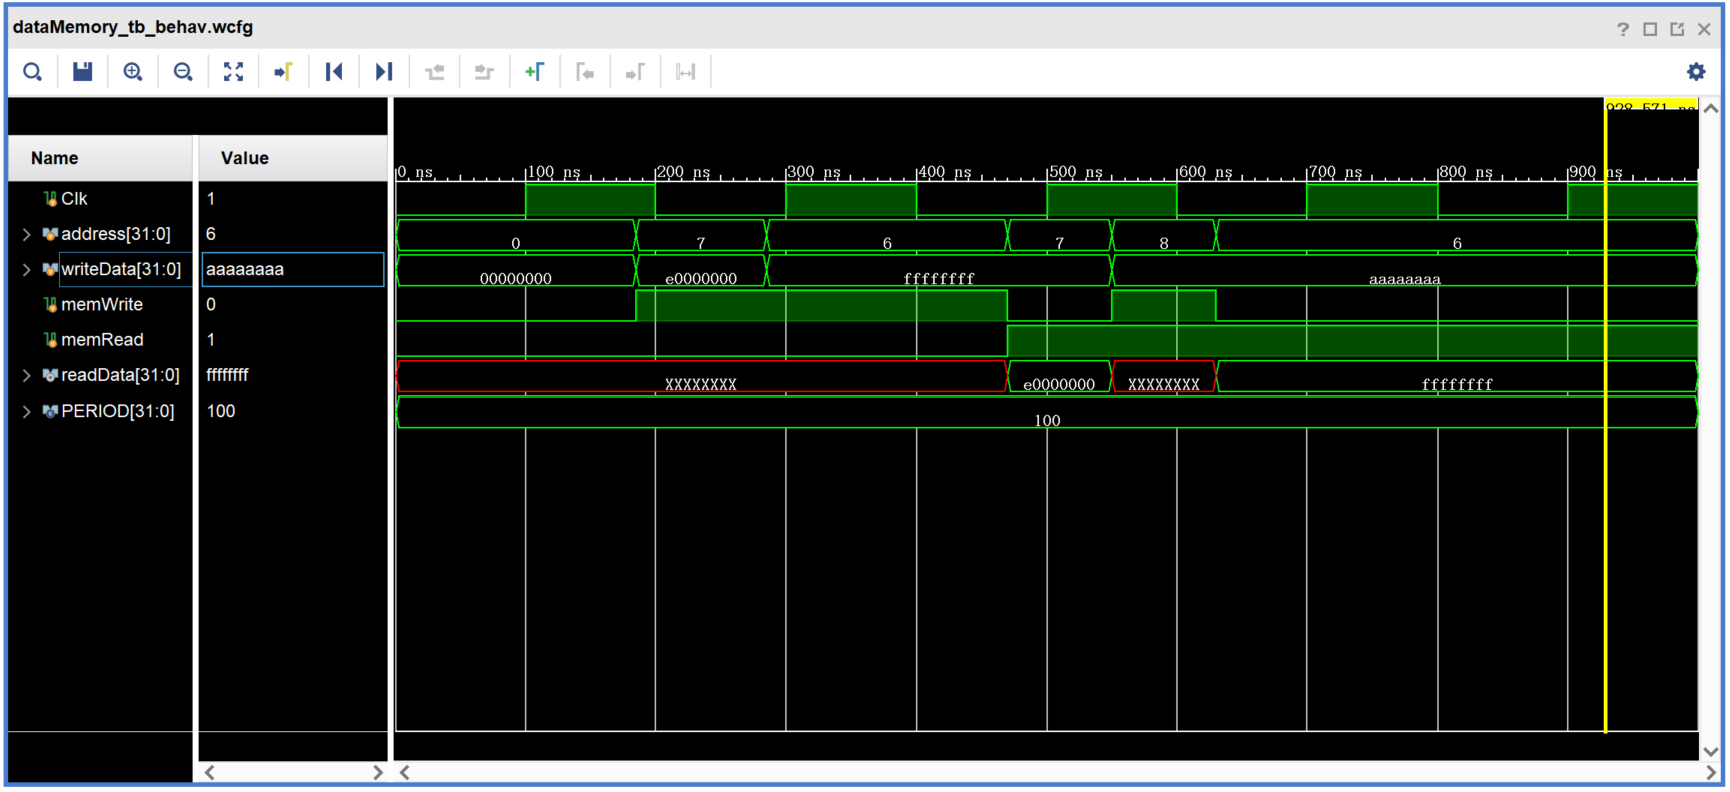
\includegraphics[width=\textwidth]{figure2.png}
    \caption{存储模块仿真结果}
    \label{fig:memtb}
\end{figure}

\subsection{带符号扩展}

带符号扩展的激励文件如下。

\begin{lstlisting}[caption=signext\_tb.v]
    initial begin
        inst = 0;
        
        #100 inst = 1;
        #100 inst = -1;
        #100 inst = 2;
        #100 inst = -2;
    end
\end{lstlisting}

带符号扩展的仿真结果如图 \ref{fig:signext} 所示。对于所有的输入,符号位扩展是正确的。
\begin{figure}[h]
    \centering
    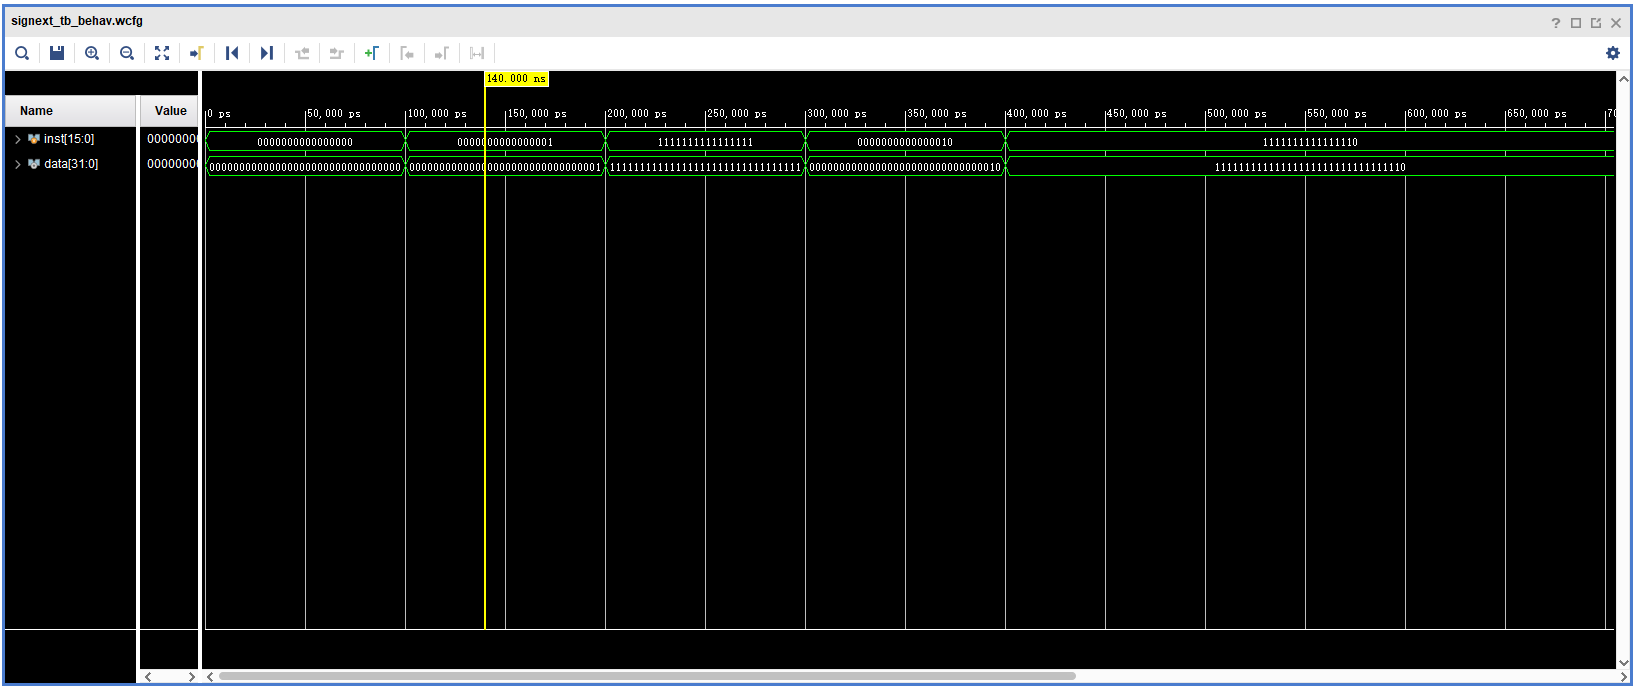
\includegraphics[width=\textwidth]{figure3.png}
    \caption{带符号扩展仿真结果}
    \label{fig:signext}
\end{figure}

\section{实验心得}

通过本次实验,更加熟悉了三个部件的构造方法。特别是时钟下沿的写入,是值得注意的。对于内存地址变化时就应当重新读取这一点也是需要特别注意的,否则会导致地址变化时无响应情形。需要注意是有效地址的内存才可以读取和写入,这一点在之后的设计中也是非常重要的。符号位扩展再次熟悉了拼接操作。

\end{document}